\section{Spectrally Heterogeneous Adaptation, Structured Forgetting}\label{sec:sensitivity}
We examine how dominant, intermediate, and trailing singular components contribute to adaptation and forgetting. Using pretrained singular values throughout, we selectively restore or retain adapted singular vectors to measure each group's contribution.

\subsection{Restoring groups of spectral components}
For a component group $B$, we restore its pretrained singular vectors and retain adapted vectors elsewhere:
\begin{equation}\label{eq:band-restore}
\bm W_{\mathrm{restore}(B)}=\bm W_{\mathrm{keep}(B^{\mathrm c})}
=\sum_{i\in B}s_{0,i}\bm u_{0,i}\bm v_{0,i}^{\!\top}
 +\sum_{i\notin B}s_{0,i}\bm u_{*,i}\bm v_{*,i}^{\!\top}.
\end{equation}

\begin{figure}[!htbp]\centering
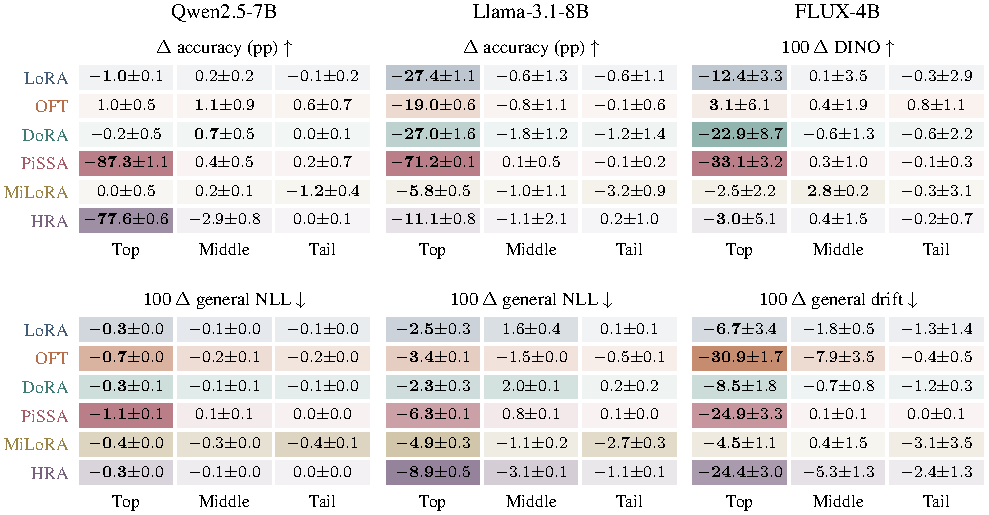
\includegraphics[width=\linewidth]{figures/peft_bands.pdf}
\caption{Dominant-component restoration consistently reduces forgetting, with varying effects on task performance. Cells show mean $\pm$ SD changes from trained models at the largest capacities and selected LRs. Higher task scores and lower NLL/drift are better. FLUX DINO/drift are scaled by 100. Bold marks the largest absolute mean change across component groups per method.}
\label{fig:band-response}
\end{figure}

\paragraph{Restoring dominant components consistently reduces forgetting.}
At the largest capacities, restoring dominant components gives the largest mean reduction in general-text NLL or general-image drift for every method (\Cref{fig:band-response}). This ordering holds across language capacities (Appendix~\ref{app:complete-interventions}). MiLoRA shares this pattern despite greater spectral drift concentration in trailing components.

\paragraph{The same restoration has different effects on task performance.}
At the largest language capacities, restoring dominant components largely preserves Qwen accuracy for LoRA, OFT, DoRA and MiLoRA, whereas PiSSA and HRA suffer large losses. The same edit reduces LoRA and DoRA accuracy by about 27 percentage points on Llama. PiSSA nearly loses all recorded accuracy on both models. In FLUX, PiSSA, LoRA and DoRA all incur substantial losses. OFT improves on average, with substantial seed variation. HRA and MiLoRA incur smaller mean losses. Thus, restoring dominant components consistently reduces forgetting, but its effect on task performance shows no consistent pattern across methods and models.

\subsection{Which components retain task performance on their own?}
Retaining only adapted dominant components preserves PiSSA's language accuracy within 1 percentage point of the full value-restored model $\bm W_R$ across every tested setting, whereas retaining only the remaining components does not. Other methods show no consistent sufficiency pattern across settings (Appendix~\ref{app:complete-interventions}, \Cref{fig:component-sufficiency,tab:capacity-sufficiency}).

\paragraph{Summary.}
Task dependence varies across settings: PiSSA’s adapted dominant components suffice across the tested settings, whereas other methods may require intermediate and trailing components. Restoring the dominant components consistently yields the largest mean reduction in NLL and drift, suggesting that forgetting is systematically associated with changes in dominant components.
